\documentclass[]{beamer}
% Class options include: notes, notesonly, handout, trans,
%                        hidesubsections, shadesubsections,
%                        inrow, blue, red, grey, brown

% Theme for beamer presentation.
\usepackage{beamerthemesplit} 
% Other themes include: beamerthemebars, beamerthemelined, 
%                       beamerthemetree, beamerthemetreebars  

\title{PHY115}    % Enter your title between curly braces
\author{Newton's Laws Of Motion}                 % Enter your name between curly braces
\institute{Digipen}      % Enter your institute name between curly braces
\date{Spring 2023} 

\begin{document}

% Creates title page of slide show using above information
\begin{frame}
  \titlepage
\end{frame}
%\note{Talk for 30 minutes} % Add notes to yourself that will be displayed when
                           % typeset with the notes or notesonly class options

\section[]{}

% Creates table of contents slide incorporating
% all \section and \subsection commands
\begin{frame}
  \tableofcontents
\end{frame}

%%%%%%%%%%%%%%%%%%%%%%%%%%%%%%%%%%%%%%%%%%%%%%%%%%%%%%%%%%%%%%%%%%%
\section{Newton's Laws Of Motion}


               \begin{frame}
NEWTON'S LAWS OF MOTION

\vspace{5mm}


\begin{itemize}
  \item Kinematics $\rightarrow$ describer motion
\item Dynamics $\rightarrow$ describes the relationship
of motion to the forces that cause it.
\end{itemize}
    
\end{frame}


%%%%%%%%%%%%%%%%%%%%%%%%%%%%%%%%%%%%%%%%%%%%%%%%%%%%%%%%%%%%%%%%%%%


\begin{frame}




Newton  deduced the three laws from
a multitude of experiments performed by other scientists, especially Galileo
Galilei.



\end{frame}
%%%%%%%%%%%%%%%%%%%%%%%%%%%%%%%%%%%%%%%%%%%%%%%%%%%%%%%%%%%%%%%%%%%
\subsection{Force}

\begin{frame}

What is a force?

\vspace{5mm}
\pause

\begin{itemize}
    \item A force is
    an interaction between two bodies or between a body and its environment.
    \item Is a vector quantity; you can push or pull a body in
    different directions.
\end{itemize}
\vspace{5mm}
\pause


\end{frame}


\begin{frame}

    There are different kinds of forces,
    
    \vspace{5mm}
    \pause
    
    \begin{itemize}
        \item Contact forces: normal force, friction force
        \item Long range forces: Gravity, Electromagnetic
    \end{itemize}
    
  


    
    
    \end{frame}

%%%%%%%%%%%%%%%%%%%%%%%%%%%%%%%%%%%%%%%%%%%%%%%%%%%%%%%%%%%%%%%%%%%


\begin{frame}

    \begin{figure}[h!]  
        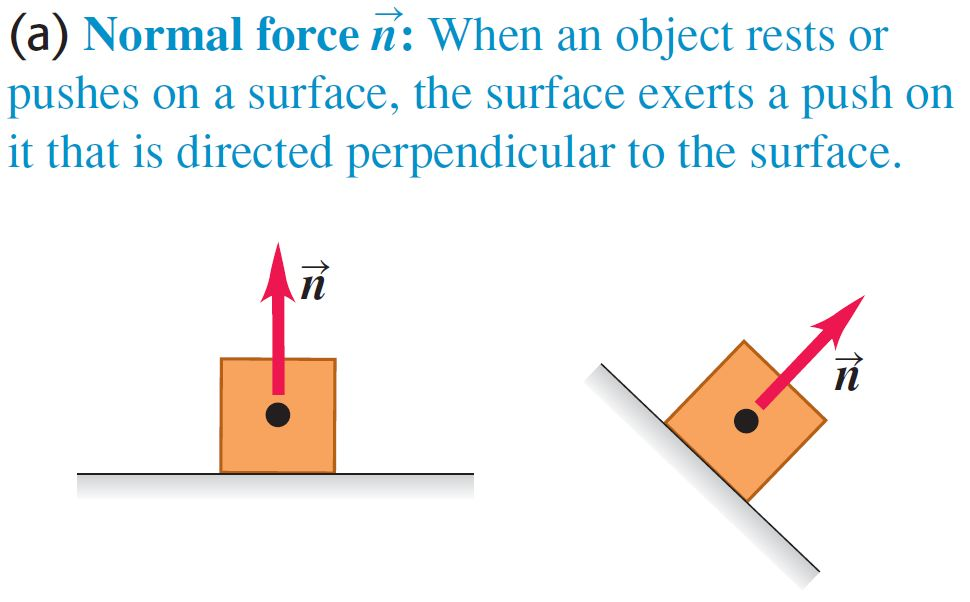
\includegraphics[width=0.8\textwidth]{images/f1.jpg}
        \caption{ {\tiny Figures from Sears and Zemansky's University Physics 
        with Modern Physics, 13th Edition.} }
      \end{figure}
  


    
    
    \end{frame}



%%%%%%%%%%%%%%%%%%%%%%%%%%%%%%%%%%%%%%%%%%%%%%%%%%%%%%%%%%%%%%%%%%%
%%%%%%%%%%%%%%%%%%%%%%%%%%%%%%%%%%%%%%%%%%%%%%%%%%%%%%%%%%%%%%%%%%%


\begin{frame}

    \begin{figure}[h!]  
        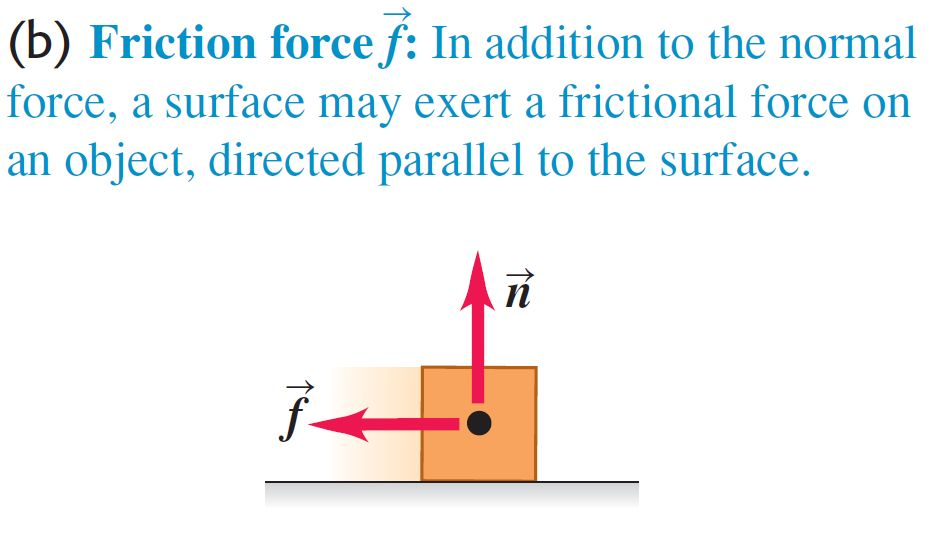
\includegraphics[width=0.8\textwidth]{images/f2.jpg}
        \caption{ {\tiny Figures from Sears and Zemansky's University Physics 
        with Modern Physics, 13th Edition.} }
      \end{figure}
  

\url{http://mw.concord.org/modeler1.3/mirror/materials/friction.html}
    


    
    \end{frame}


%%%%%%%%%%%%%%%%%%%%%%%%%%%%%%%%%%%%%%%%%%%%%%%%%%%%%%%%%%%%%%%%%%%


\begin{frame}

  \begin{figure}[h!]  
      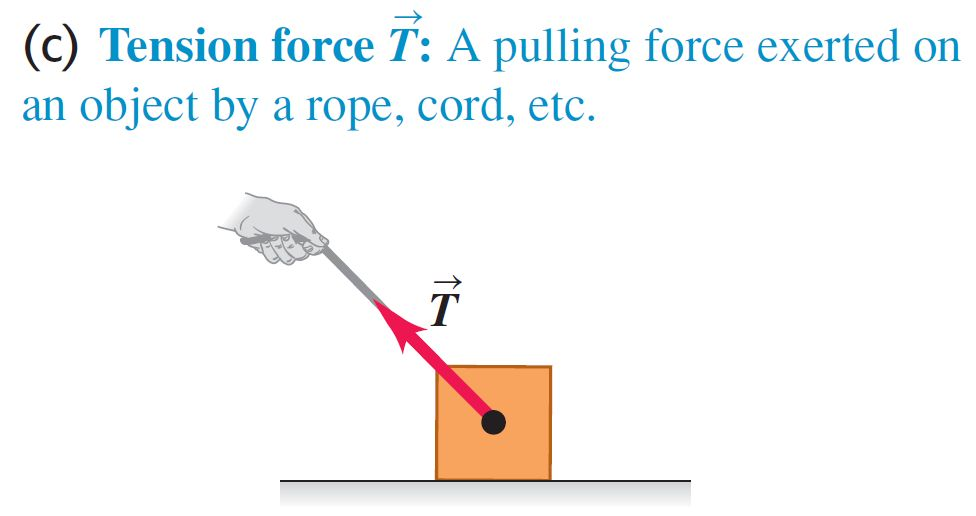
\includegraphics[width=0.8\textwidth]{images/f3.jpg}
      \caption{ {\tiny Figures from Sears and Zemansky's University Physics 
      with Modern Physics, 13th Edition.} }
    \end{figure}



  
  
  \end{frame}

  


    

%%%%%%%%%%%%%%%%%%%%%%%%%%%%%%%%%%%%%%%%%%%%%%%%%%%%%%%%%%%%%%%%%%%


\begin{frame}

    \begin{figure}[h!]  
        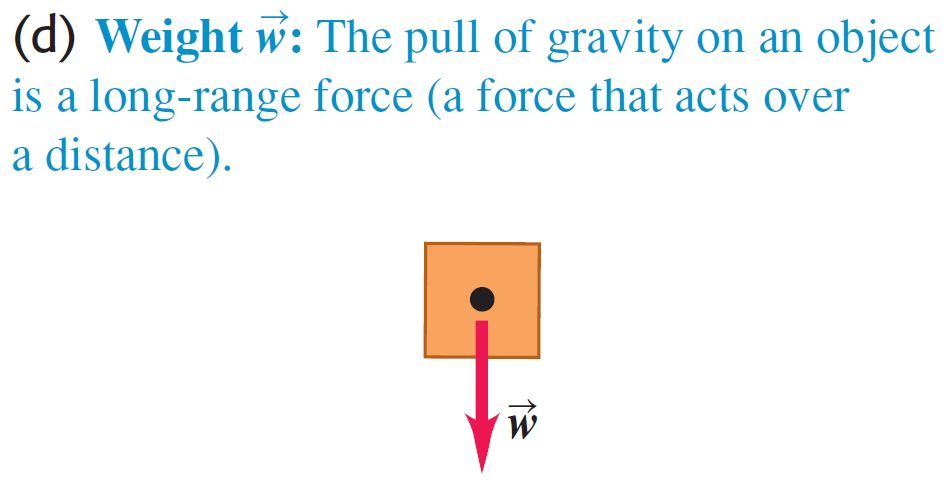
\includegraphics[width=0.8\textwidth]{images/f4.jpg}
        \caption{ {\tiny Figure from Sears and Zemansky's University Physics 
        with Modern Physics, 13th Edition.} }
      \end{figure}
    
    \end{frame}





%%%%%%%%%%%%%%%%%%%%%%%%%%%%%%%%%%%%%%%%%%%%%%%%%%%%%%%%%%%%%%%%%%%


\begin{frame}

The units of force are Newtons.    
 

\begin{figure}[h!]  
  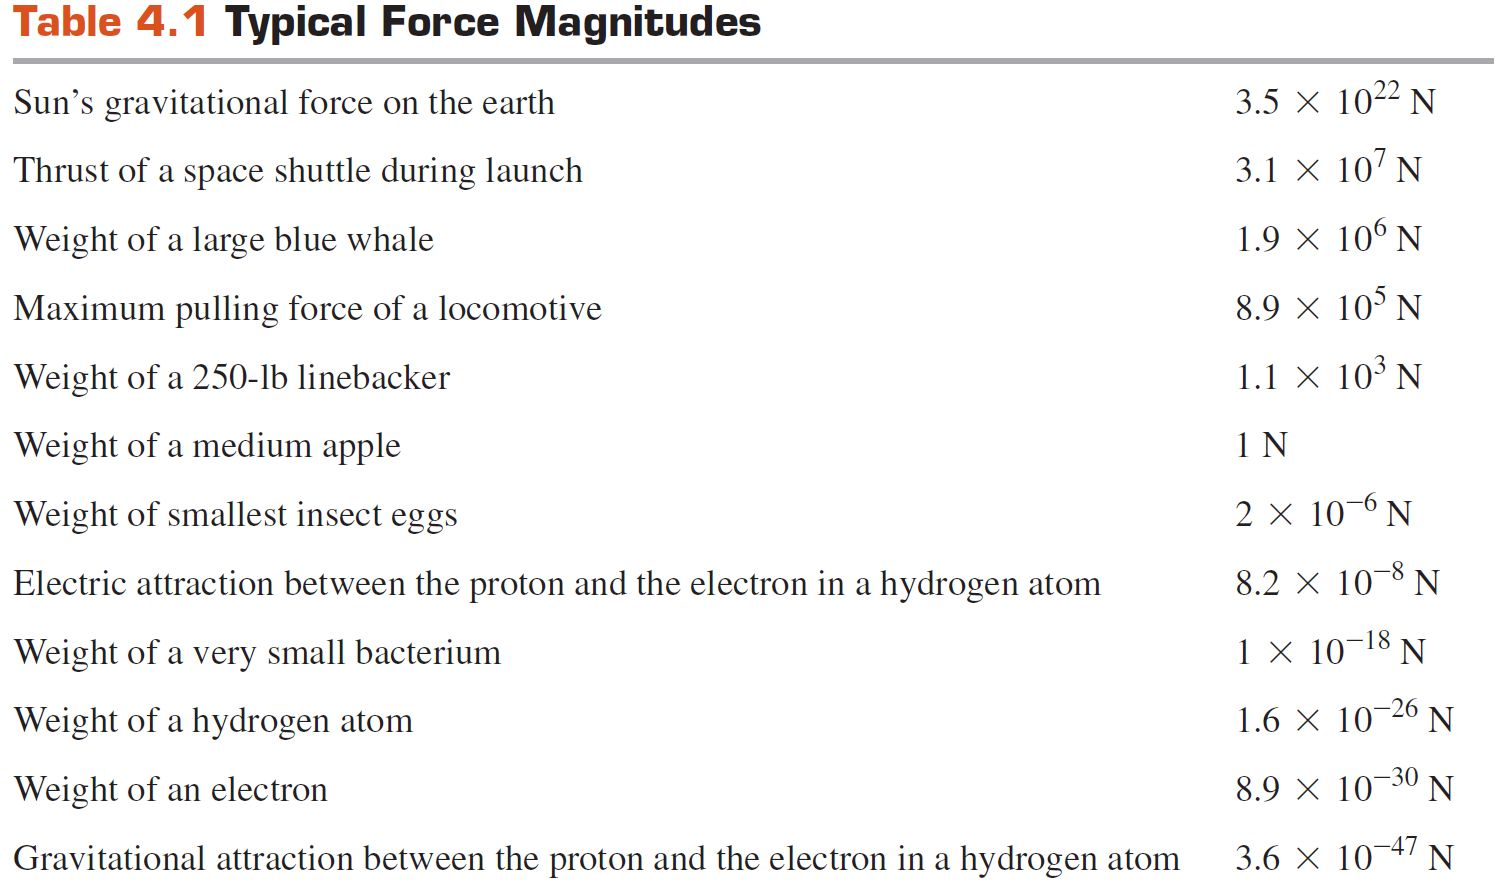
\includegraphics[width=1.\textwidth]{images/f5.jpg}
  \caption{ {\tiny Figures from Sears and Zemansky's University Physics 
  with Modern Physics, 13th Edition.} }
\end{figure}


    
    \end{frame}
%%%%%%%%%%%%%%%%%%%%%%%%%%%%%%%%%%%%%%%%%%%%%%%%%%%%%%%%%%%%%%%%%%%

\begin{frame}

 Superposition of Forces
         
 \begin{figure}[h!]  
  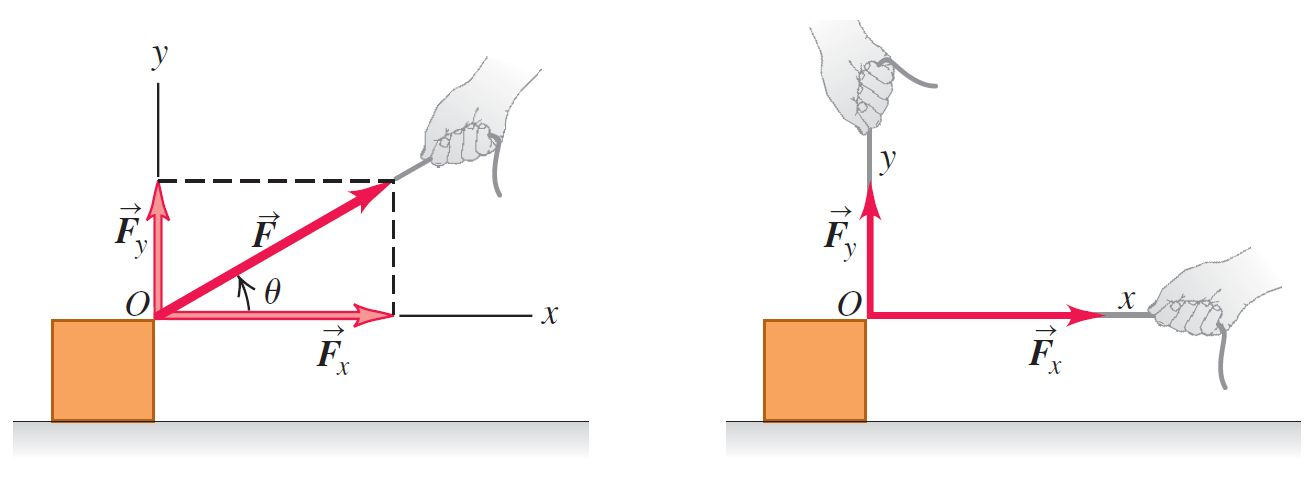
\includegraphics[width=1.\textwidth]{images/f6.jpg}
  \caption{ {\tiny Figures from Sears and Zemansky's University Physics 
  with Modern Physics, 13th Edition.} }
\end{figure}


  
    \begin{equation}
      \vec{R}=\vec{F}_1+\vec{F}_2+\vec{F}_3+\cdot=\sum \vec{F}
    \end{equation}
    
      \pause
   In 2D:
   
   \begin{equation}
    R_x=\sum F_x,~R_y=\sum F_y,~R=\sqrt{R^2_x+R^2_y}
   \end{equation}
      
      \end{frame}
  



%%%%%%%%%%%%%%%%%%%%%%%%%%%%%%%%%%%%%%%%%%%%%%%%%%%%%%%%%%%%%%%%%%%
\begin{frame}

  Example: What bis the resultant Force?
    
\begin{figure}[h!]  
   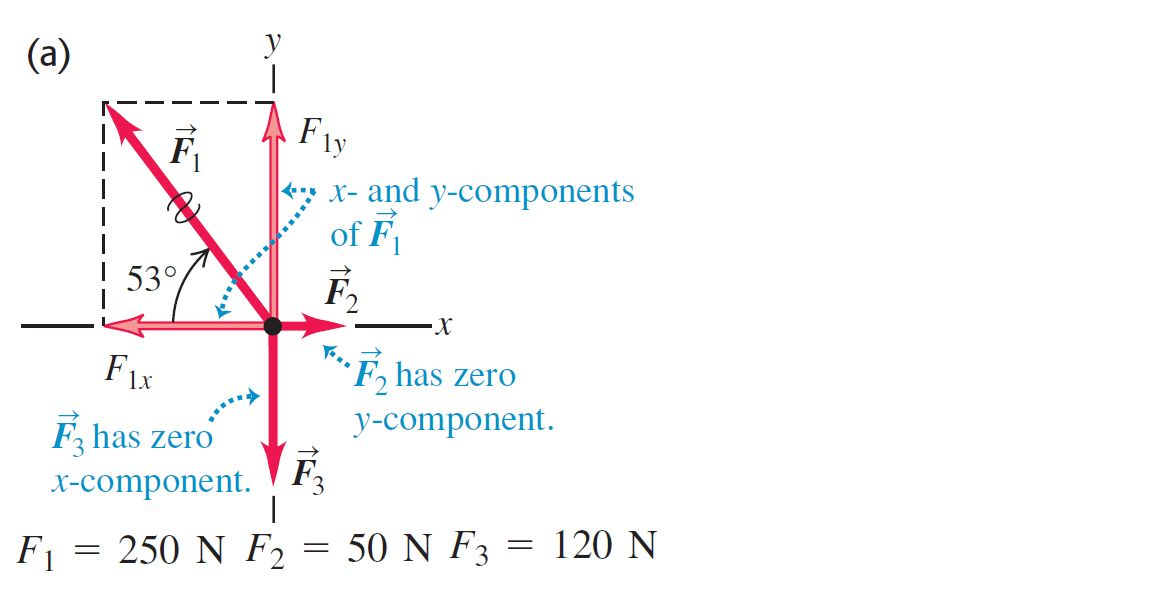
\includegraphics[width=1.\textwidth]{images/f7.jpg}
   \caption{ {\tiny Figures from Sears and Zemansky's University Physics 
   with Modern Physics, 13th Edition.} }
 \end{figure}
 
\end{frame}
  



%%%%%%%%%%%%%%%%%%%%%%%%%%%%%%%%%%%%%%%%%%%%%%%%%%%%%%%%%%%%%%%%%%%
\begin{frame}

  Example: What bis the resultant Force?
    
       
  \begin{figure}[h!]  
   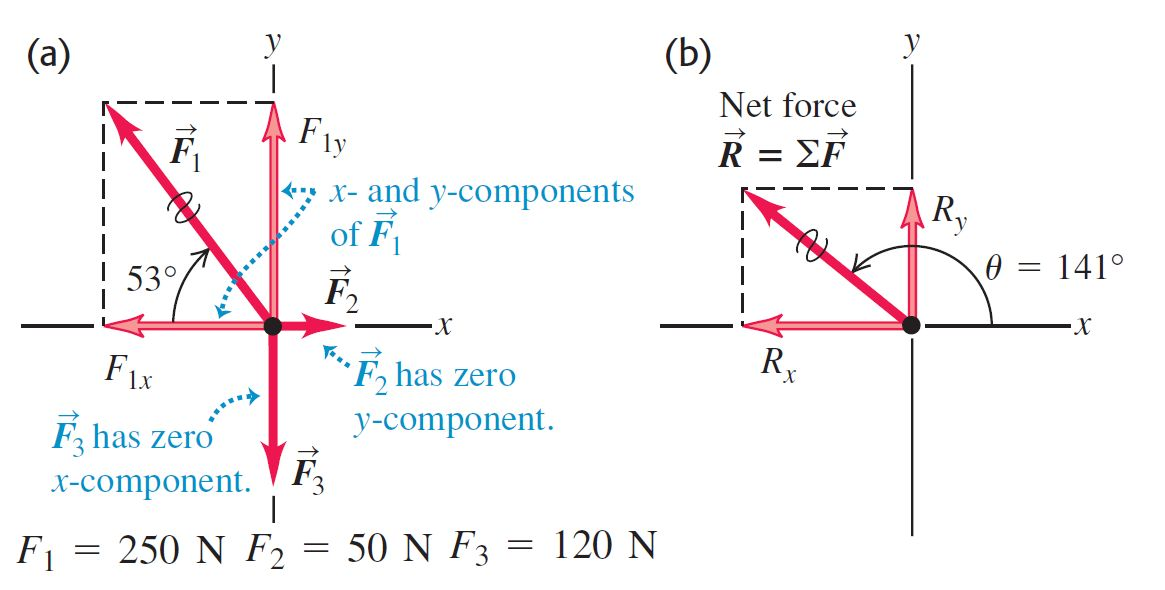
\includegraphics[width=1.\textwidth]{images/f8.jpg}
   \caption{ {\tiny Figures from Sears and Zemansky's University Physics 
   with Modern Physics, 13th Edition.} }
 \end{figure}
 
 \end{frame}
   
%%%%%%%%%%%%%%%%%%%%%%%%%%%%%%%%%%%%%%%%%%%%%%%%%%%%%%%%%%%%%%%%%%%



 \begin{frame}

 With the x- and y-axes shown in the figure, which statement
 about the components of the gravitational force that the earth exerts on the crate
 (the crate’s weight) is correct? 
 \vspace{3mm}

\begin{enumerate}
  \item The x- and y-components are both positive.
  \item The x-component is zero and the y-component is positive.
  \item The x-component is negative   and the y-component is positive.
  \item The x- and y-components are both negative.
  \item The x-component is zero and the y-component is negative.
  \item The x-component is   positive and the y-component is negative.
\end{enumerate}


 \begin{figure}[h!]  
  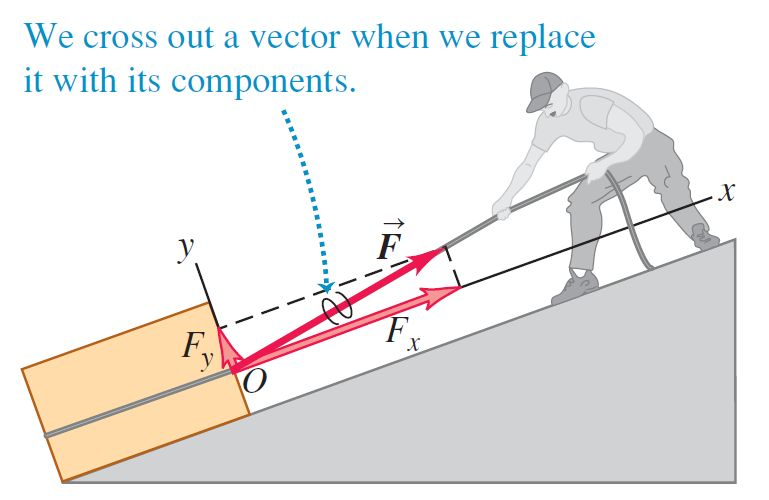
\includegraphics[width=0.4\textwidth]{images/f9.jpg}
  \caption{ {\tiny Figures from Sears and Zemansky's University Physics 
  with Modern Physics, 13th Edition.} }
\end{figure}


\end{frame}


 %%%%%%%%%%%%%%%%%%%%%%%%%%%%%%%%%%%%%%%%%%%%%%%%%%%%%%%%%%%%%%%%%%%
\subsection{Newton's First Law}
 \begin{frame}

How do the forces that act on a body affect its motion?
 \pause

 \vspace{5mm}
What common sense says? 
\pause

\vspace{5mm}

\textit{"Objects do not continue to move indefinitely; they slow
down and stop unless there is a force that sustain the motion"...}

\vspace{5mm}
\pause
THIS STATEMENT IS WRONG !!
 
 \end{frame}


 %%%%%%%%%%%%%%%%%%%%%%%%%%%%%%%%%%%%%%%%%%%%%%%%%%%%%%%%%%%%%%%%%%%
 \begin{frame}

NEWTON'S FIRST LAW
\vspace{5mm}

 \begin{enumerate}
   \item A body acted on by no net force moves with
   constant velocity (which may be zero) and zero acceleration.
 \end{enumerate}
  \pause

 The tendency of a body to keep moving once it is set in motion results from a
 property called \textbf{inertia}.
 
 \end{frame}



 %%%%%%%%%%%%%%%%%%%%%%%%%%%%%%%%%%%%%%%%%%%%%%%%%%%%%%%%%%%%%%%%%%%
 \begin{frame}
 Equilibrium
  \vspace{5mm}

  When a body is either at rest or moving with constant velocity (in a straight
  line with constant speed), we say that the body is in \textbf{equilibrium}.

  \begin{equation*}
    \sum \vec{F}=\textbf{0}\rightarrow \sum F_x=0~and~\sum F_y=0
  \end{equation*}
   


   \end{frame}


 %%%%%%%%%%%%%%%%%%%%%%%%%%%%%%%%%%%%%%%%%%%%%%%%%%%%%%%%%%%%%%%%%%%
 \begin{frame}
  Inertial Frame of Reference
    \vspace{5mm}
  
  
    This concept is central to Newton’s laws of motion.
    \vspace{5mm}
    \pause

    Let's see this example of motion inside the International Space Station:

    \vspace{5mm}

\url{https://www.youtube.com/watch?v=d1iO-yDp_nA}
     
\pause
   \vspace{5mm}


In the Previous example, Newton's First law seems not to be working! 
  
\end{frame}
 %%%%%%%%%%%%%%%%%%%%%%%%%%%%%%%%%%%%%%%%%%%%%%%%%%%%%%%%%%%%%%%%%%%


 \begin{frame}
  Inertial Frame of Reference
    \vspace{5mm}
  

Newton's First Law is valid in some frames of reference and not valid in others. 
\vspace{3mm}
\pause

A frame of reference in which Newton’s first law is valid is called an inertial frame of
 reference.
 \vspace{3mm}
\pause

The earth is at least approximately an inertial frame of reference,

\vspace{3mm}
\pause

An inertial frame of reference is a frame of reference that is not undergoing acceleration.

\vspace{3mm}
\pause
We name the apparent forces that act on bodies in a non-inertial reference frame, 
\textbf{Fictitious Forces}.

\end{frame}



%%%%%%%%%%%%%%%%%%%%%%%%%%%%%%%%%%%%%%%%%%%%%%%%%%%%%%%%%%%%%%%%%%%


\begin{frame}
Non-Inertial Frames of References

\vspace{5mm}
  
\begin{itemize}
\item Rotating surfaces.
\item Accelerating cars.
\item ...
\end{itemize}
\end{frame}



%%%%%%%%%%%%%%%%%%%%%%%%%%%%%%%%%%%%%%%%%%%%%%%%%%%%%%%%%%%%%%%%%%%


\begin{frame}

  There are many inertial frames...


  \vspace{5mm}
  \pause

  If we have an inertial frame  of reference A, in which Newton’s first law is obeyed, then any second frame
  of reference B will also be inertial if it moves relative to A with constant   velocity.

  \begin{columns}[c]
    \column{2in}  % slides are 3in high by 5in wide
       
    \begin{figure}[h!]  
      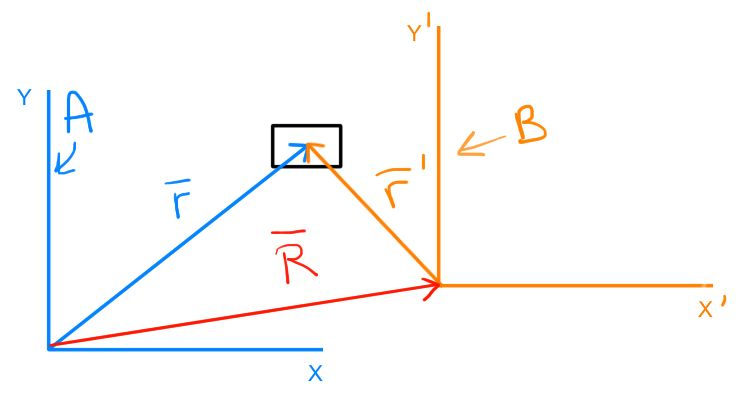
\includegraphics[width=1.2\textwidth]{images/f10.jpg}
     
    \end{figure}

    \column{2in}
 
    \begin{equation*}
      \vec{r}=\vec{R}+\vec{r'}\rightarrow \vec{v}=\vec{V}+\vec{v'}
    \end{equation*}

    \begin{equation*}
    \rightarrow \vec{a}=\vec{A}+\vec{a'}
    \end{equation*}


    
    \begin{equation*}
     if~\vec{A}=\vec{0}\rightarrow \vec{a}=\vec{a'}
      \end{equation*}

  
    \end{columns}
 


     \end{frame}




%%%%%%%%%%%%%%%%%%%%%%%%%%%%%%%%%%%%%%%%%%%%%%%%%%%%%%%%%%%%%%%%%%%


\begin{frame}

  Test Your Understanding 
  \vspace{3mm}
  
  In which of the following  situations is there zero net force on the body? 
  
  \begin{enumerate}
    \item an airplane flying due north at a steady $120~m/s$ and at a constant altitude;
    \item a car driving straight up a hill with a $3\deg$ slope at a constant $90~km/h$:
    \item a hawk circling at a constant speed at a constant height of 15 m above an open field;
    \item  a box with slick, frictionless surfaces in the back of a truck as the truck 
    accelerates forward on a level road at $5 m/s^ 2$.
  \end{enumerate}
  
  
 
     \end{frame}

%%%%%%%%%%%%%%%%%%%%%%%%%%%%%%%%%%%%%%%%%%%%%%%%%%%%%%%%%%%%%%%%%%%

\subsection{  Newton's Second Law }
\begin{frame}

 Newton's Second Law 
  \vspace{3mm}
  
  Experiments shows that a net force acting on a body causes the body to accelerate in
  the same direction as the net force.
  \vspace{3mm}
 
\pause
\vspace{5mm}


Then, the relation between the acceleration and Force that produces it, must be something like\dots

\begin{equation}
  \sum\vec{F}=(positive~number)\cdot \vec{a}
\end{equation}


     \end{frame}


%%%%%%%%%%%%%%%%%%%%%%%%%%%%%%%%%%%%%%%%%%%%%%%%%%%%%%%%%%%%%%%%%%%

\begin{frame}

Mass and Force

\vspace{5mm}
Then for a given body, we have:
\pause

\begin{equation*}
  (positive~number)= \frac{\vert\sum\vec{F}\vert}{\vert\vec{a}\vert}
\end{equation*}
\pause

We call this positive number \textit{the inertial mass}, or simply the
\textbf{mass} $m$.

\pause

\begin{equation}
 \boxed{m= \frac{\vert\sum\vec{F}\vert}{\vert\vec{a}\vert}}
\end{equation}

     \end{frame}


%%%%%%%%%%%%%%%%%%%%%%%%%%%%%%%%%%%%%%%%%%%%%%%%%%%%%%%%%%%%%%%%%%%

\begin{frame}

If we measure the mass in $kg$, 
\vspace{5mm}

\pause
One newton is the amount of net force that gives an acceleration of 1 meter per
second squared to a body with a mass of 1 kilogram.
\pause
\vspace{5mm}

\begin{equation}
  \boxed{1~N=1~kg\cdot m/s^ 2}
 \end{equation}
  
\end{frame}


%%%%%%%%%%%%%%%%%%%%%%%%%%%%%%%%%%%%%%%%%%%%%%%%%%%%%%%%%%%%%%%%%%%

\begin{frame}
Stating Newton's Second law
\pause
\vspace{5mm}

If a net external force acts on a body, the
body accelerates. The direction of acceleration is the same as the direction of the
net force. The mass of the body times the acceleration of the body equals the net
force vector.
\pause
\vspace{5mm}


\begin{equation}
  \boxed{\sum\vec{F}=m\cdot \vec{a}}
\end{equation}

\vspace{5mm}


\begin{equation*}
 \sum F_x=m a_x,~\sum F_y=m a_y,~\sum F_z=m a_z 
\end{equation*}
\pause
\vspace{5mm}

This is only valid when the mass is constant.

\pause
Example: \url{https://www.youtube.com/watch?v=sPZ2bjW53c8}

    \end{frame}



%%%%%%%%%%%%%%%%%%%%%%%%%%%%%%%%%%%%%%%%%%%%%%%%%%%%%%%%%%%%%%%%%%%

\begin{frame}

  \boxed{CAUTION }
  \vspace{5mm}
  
 $m\cdot \vec{a}$ is not a force. You must keep in mind that even though the vector is
  equal to the vector sum of all the forces acting on the body, the vector is not a
  force. Acceleration is a result of a nonzero net force; it is not a force itself. 
  \pause
  
  
    \end{frame}



%%%%%%%%%%%%%%%%%%%%%%%%%%%%%%%%%%%%%%%%%%%%%%%%%%%%%%%%%%%%%%%%%%%




\begin{frame}

 Mass and Weight
 \vspace{5mm}

\begin{itemize}
  \item  Mass characterizes the inertial properties of a body.
  \item The greater the mass, the greater the force needed to cause a given acceleration.
  \item Weight, on the other hand, is a force exerted on a body by the pull of the earth.
\end{itemize}
  

\begin{equation}
  \vec{w}=m\vec{g}
\end{equation}

If the mass is $1~kg$, then
\begin{equation}
  w=ma=(1~kg)(9.8~m/s^2)=9.8~N
\end{equation}
  
  \end{frame}

    %%%%%%%%%%%%%%%%%%%%%%%%%%%%%%%%%%%%%%%%%%%%%%%%%%%%%%%%%%%%%%%%%%%


\begin{frame}
  Measuring Mass and Weight
  \vspace{5mm}

We can measure mass comparing its weight to a known weight.


The standard mass is defined as the mass  f a cylinder of platinum–iridium alloy 
kept in a vault near Paris.




\begin{figure}[h!]  
  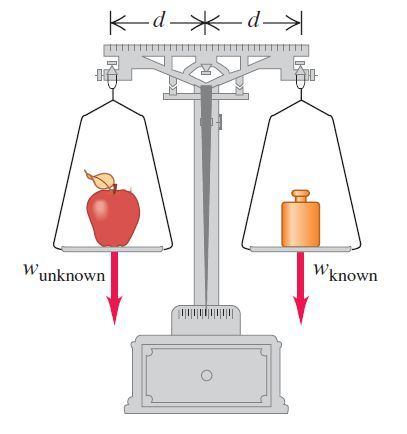
\includegraphics[width=0.5\textwidth]{images/f11.jpg}
  \caption{ {\tiny Figures from Sears and Zemansky's University Physics 
  with Modern Physics, 13th Edition.} }
\end{figure}




  \end{frame}



    %%%%%%%%%%%%%%%%%%%%%%%%%%%%%%%%%%%%%%%%%%%%%%%%%%%%%%%%%%%%%%%%%%%

\subsection{ Newton’s Third Law}

    \begin{frame}
      Newton’s Third Law
      \vspace{5mm}
    
      If body A exerts a force on body B (an
      “action”), then body B exerts a force on body A (a “reaction”). These two forces
      have the same magnitude but are opposite in direction. These two forces act on
      different bodies.
    
      \begin{equation}
        \vec{F}_{A~ on ~ B}=-\vec{F}_{B~ on ~ A}
      \end{equation}
    
      \vspace{5mm}

      Example \url{https://www.youtube.com/watch?v=ZkVU-bj9bDk}



      \end{frame}


  %%%%%%%%%%%%%%%%%%%%%%%%%%%%%%%%%%%%%%%%%%%%%%%%%%%%%%%%%%%%%%%%%%%


  \begin{frame}
  

    Example, what is wrong in this scene?
    
    
    \url{https://www.youtube.com/watch?v=dKJa-KQNjQU}



    \end{frame}

    %%%%%%%%%%%%%%%%%%%%%%%%%%%%%%%%%%%%%%%%%%%%%%%%%%%%%%%%%%%%%%%%%%%

  

    \begin{frame}
      An apple sits at rest on a table, in equilibrium. What forces act on
      the apple? What is the reaction force to each of the forces acting on
      the apple? Which are the action–reaction pairs?
      \vspace{5mm}
    

      \begin{figure}[h!]  
        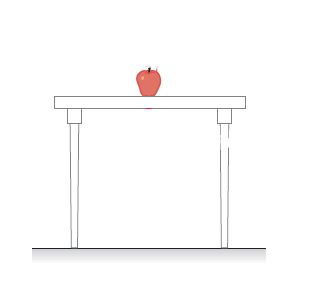
\includegraphics[width=0.5\textwidth]{images/f12.jpg}
        \caption{ {\tiny Figures from Sears and Zemansky's University Physics 
        with Modern Physics, 13th Edition.} }
      \end{figure}

      \end{frame}










    %%%%%%%%%%%%%%%%%%%%%%%%%%%%%%%%%%%%%%%%%%%%%%%%%%%%%%%%%%%%%%%%%%%

    

    \begin{frame}
      Identify the forces that act when a mason pulls on a rope attached to a block.
      \vspace{5mm}
    

      \begin{figure}[h!]  
        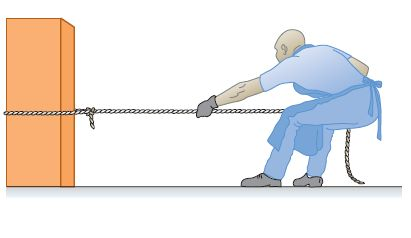
\includegraphics[width=0.5\textwidth]{images/f13.jpg}
        \caption{ {\tiny Figures from Sears and Zemansky's University Physics 
        with Modern Physics, 13th Edition.} }
      \end{figure}

      \end{frame}





    %%%%%%%%%%%%%%%%%%%%%%%%%%%%%%%%%%%%%%%%%%%%%%%%%%%%%%%%%%%%%%%%%%%

 

    \begin{frame}
      The stonemason pulls as hard on the rope–block combination as that combination pulls
      back on him. Why, then, does the block move while the stonemason  remains stationary?
      
      \vspace{5mm}
    

      \begin{figure}[h!]  
        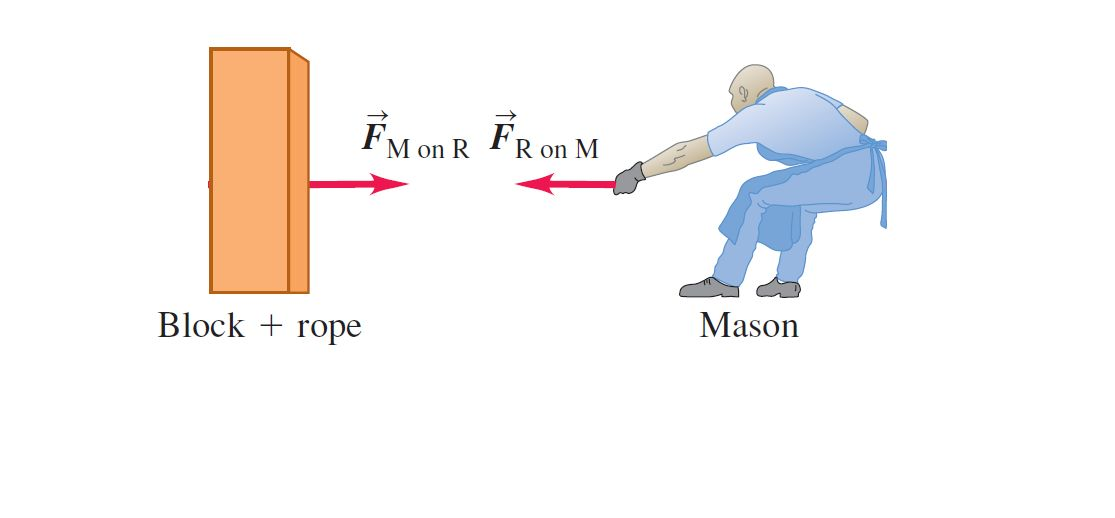
\includegraphics[width=1.\textwidth]{images/f15.jpg}
        \caption{ {\tiny Figures from Sears and Zemansky's University Physics 
        with Modern Physics, 13th Edition.} }
      \end{figure}

      \end{frame}



    %%%%%%%%%%%%%%%%%%%%%%%%%%%%%%%%%%%%%%%%%%%%%%%%%%%%%%%%%%%%%%%%%%%

%  \subsection{Free-Body Diagrams}

    \begin{frame}
      \begin{itemize}
        \item Choose a body, identify all the forces acting on it. 
        \item Draw them as vectors
        \item Apply Newton's Second Law $\sum \vec{F}=m\vec{a}$
      \end{itemize}
      \end{frame}


    %%%%%%%%%%%%%%%%%%%%%%%%%%%%%%%%%%%%%%%%%%%%%%%%%%%%%%%%%%%%%%%%%%%


    \begin{frame}
 Example, which force makes you walk? 
 \vspace{3mm}

 \url{https://www.youtube.com/watch?v=G8Veye-N0A4}

      \end{frame}





    %%%%%%%%%%%%%%%%%%%%%%%%%%%%%%%%%%%%%%%%%%%%%%%%%%%%%%%%%%%%%%%%%%%


    \begin{frame}
Example, an inclined plane.
\vspace{3mm}


A car of weight $w$ rests on a slanted ramp attached to a trailer.
 Only a cable running from the trailer to the car prevents
the car from rolling off the ramp. (The car’s brakes are off and its transmission is in neutral.) Find the tension in the cable
and the force that the ramp exerts on the car’s tires.


\begin{figure}[h!]  
  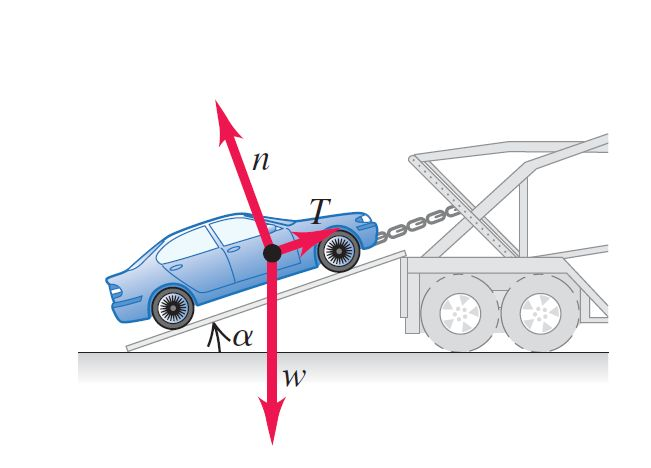
\includegraphics[width=0.4\textwidth]{images/f16.jpg}
  \caption{ {\tiny Figures from Sears and Zemansky's University Physics 
  with Modern Physics, 13th Edition.} }
\end{figure}



      \end{frame}



    %%%%%%%%%%%%%%%%%%%%%%%%%%%%%%%%%%%%%%%%%%%%%%%%%%%%%%%%%%%%%%%%%%%


    \begin{frame}
Example, tension in an elevator cable
\vspace{3mm}


An elevator and its load have a combined mass of 800 kg.
The elevator is initially moving downward at $10~m/s$ it slows to
a stop with constant acceleration in a distance of $25 m$. What is
the tension T in the supporting cable while the elevator is being
brought to rest?

\begin{figure}[h!]  
  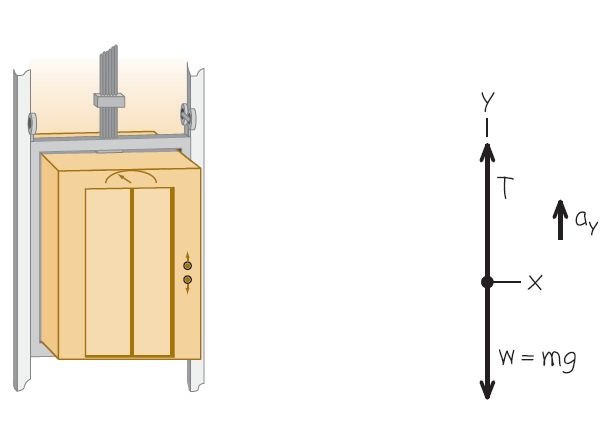
\includegraphics[width=0.5\textwidth]{images/f17.jpg}
  \caption{ {\tiny Figures from Sears and Zemansky's University Physics 
  with Modern Physics, 13th Edition.} }
\end{figure}



      \end{frame}


    %%%%%%%%%%%%%%%%%%%%%%%%%%%%%%%%%%%%%%%%%%%%%%%%%%%%%%%%%%%%%%%%%%%


    \begin{frame}
      
What happend when $a_y=-g$?
\vspace{3mm}



\begin{figure}[h!]  
  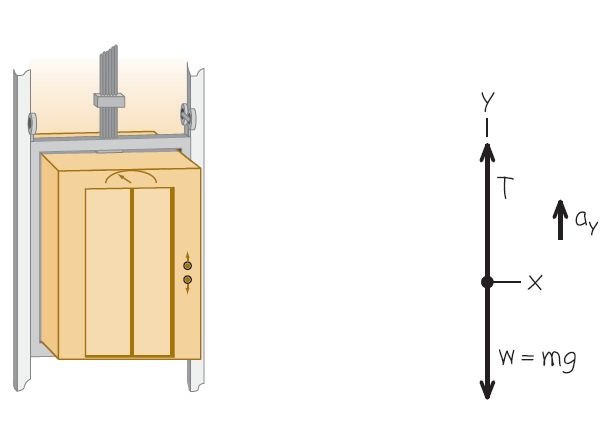
\includegraphics[width=0.4\textwidth]{images/f17.jpg}
  \caption{ {\tiny Figures from Sears and Zemansky's University Physics 
  with Modern Physics, 13th Edition.} }
\end{figure}

\pause
Apparent weightlessness


      \end{frame}




    %%%%%%%%%%%%%%%%%%%%%%%%%%%%%%%%%%%%%%%%%%%%%%%%%%%%%%%%%%%%%%%%%%%


    \begin{frame}
      
      A toboggan loaded with students (total weight w) slides down a
      snow-covered slope. The hill slopes at a constant angle, and the
      toboggan is so well waxed that there is virtually no friction. What
      is its acceleration?

      \begin{figure}[h!]  
        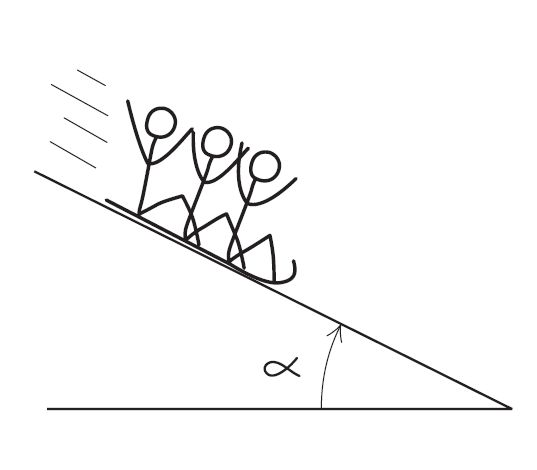
\includegraphics[width=0.5\textwidth]{images/f18.jpg}
        \caption{ {\tiny Figures from Sears and Zemansky's University Physics 
        with Modern Physics, 13th Edition.} }
      \end{figure}


      \end{frame}



    %%%%%%%%%%%%%%%%%%%%%%%%%%%%%%%%%%%%%%%%%%%%%%%%%%%%%%%%%%%%%%%%%%%


    \begin{frame}
      
  Frictional Forces
\vspace{3mm}



\begin{itemize}
  \item The  friction force arises from interactions between molecules
  on the surfaces of two bodies.
  \item The higher the normal force, the higher are the interactions $\rightarrow$ the higher is the friction force.
\end{itemize}


\begin{figure}[h!]  
  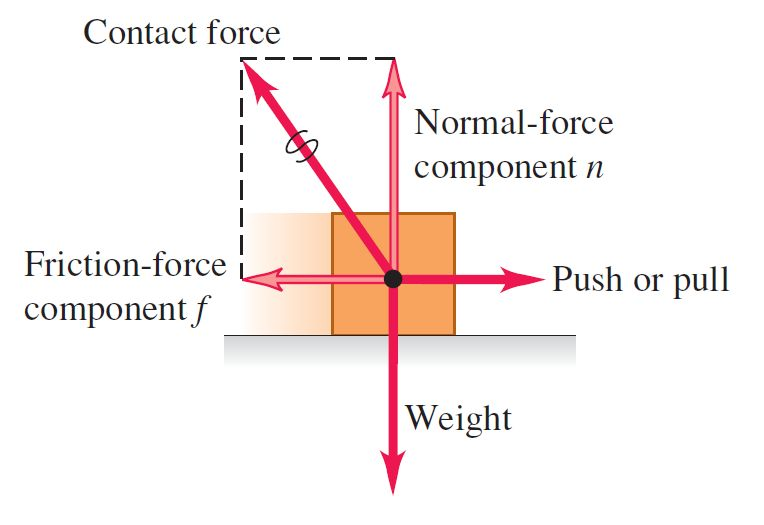
\includegraphics[width=0.5\textwidth]{images/f19.jpg}
  \caption{ {\tiny Figures from Sears and Zemansky's University Physics 
  with Modern Physics, 13th Edition.} }
\end{figure}
      \end{frame}



    %%%%%%%%%%%%%%%%%%%%%%%%%%%%%%%%%%%%%%%%%%%%%%%%%%%%%%%%%%%%%%%%%%%


    \begin{frame}
      
      Frictional Forces
    \vspace{3mm}
    
\begin{equation}
  f_k=\mu_k N
\end{equation}
   

          \vspace{3mm}
    
          \begin{figure}[h!]  
            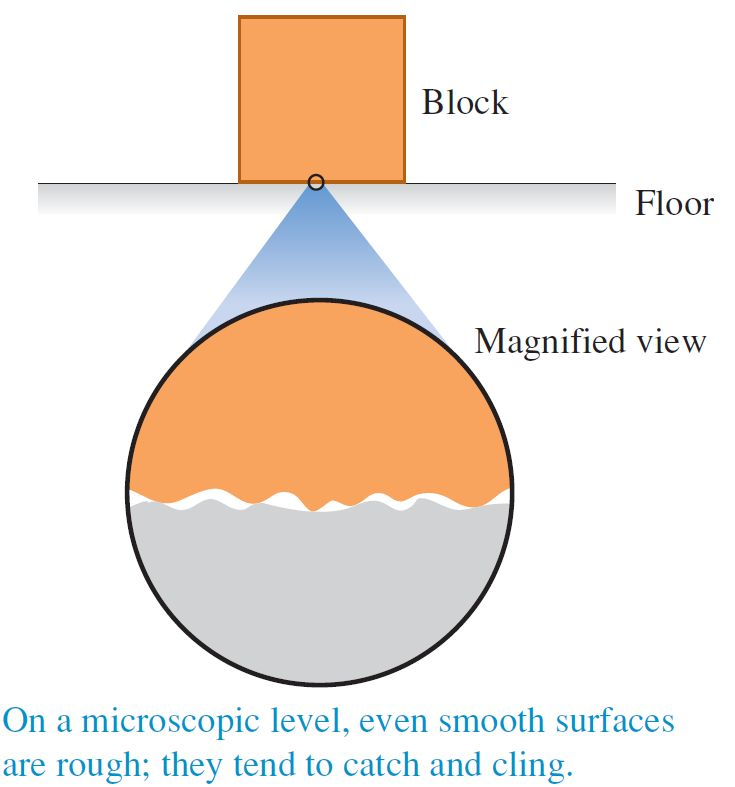
\includegraphics[width=0.4\textwidth]{images/f22.jpg}
            \caption{ {\tiny Table from Sears and Zemansky's University Physics 
            with Modern Physics, 13th Edition.} }
          \end{figure}


        \end{frame}


    %%%%%%%%%%%%%%%%%%%%%%%%%%%%%%%%%%%%%%%%%%%%%%%%%%%%%%%%%%%%%%%%%%%


    \begin{frame}
      
 Coefficients of Friction
    \vspace{3mm}
    
    \begin{figure}[h!]  
      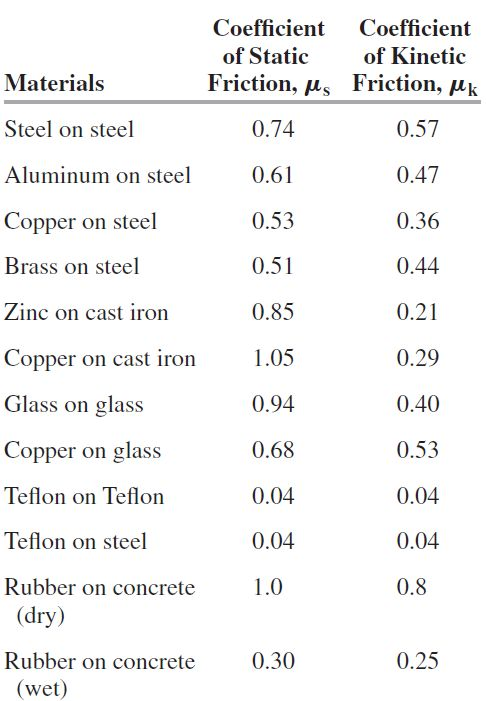
\includegraphics[width=0.4\textwidth]{images/f20.jpg}
      \caption{ {\tiny Table from Sears and Zemansky's University Physics 
      with Modern Physics, 13th Edition.} }
    \end{figure}

          \end{frame}






    %%%%%%%%%%%%%%%%%%%%%%%%%%%%%%%%%%%%%%%%%%%%%%%%%%%%%%%%%%%%%%%%%%%


    \begin{frame}
      
 
         
         \begin{figure}[h!]  
           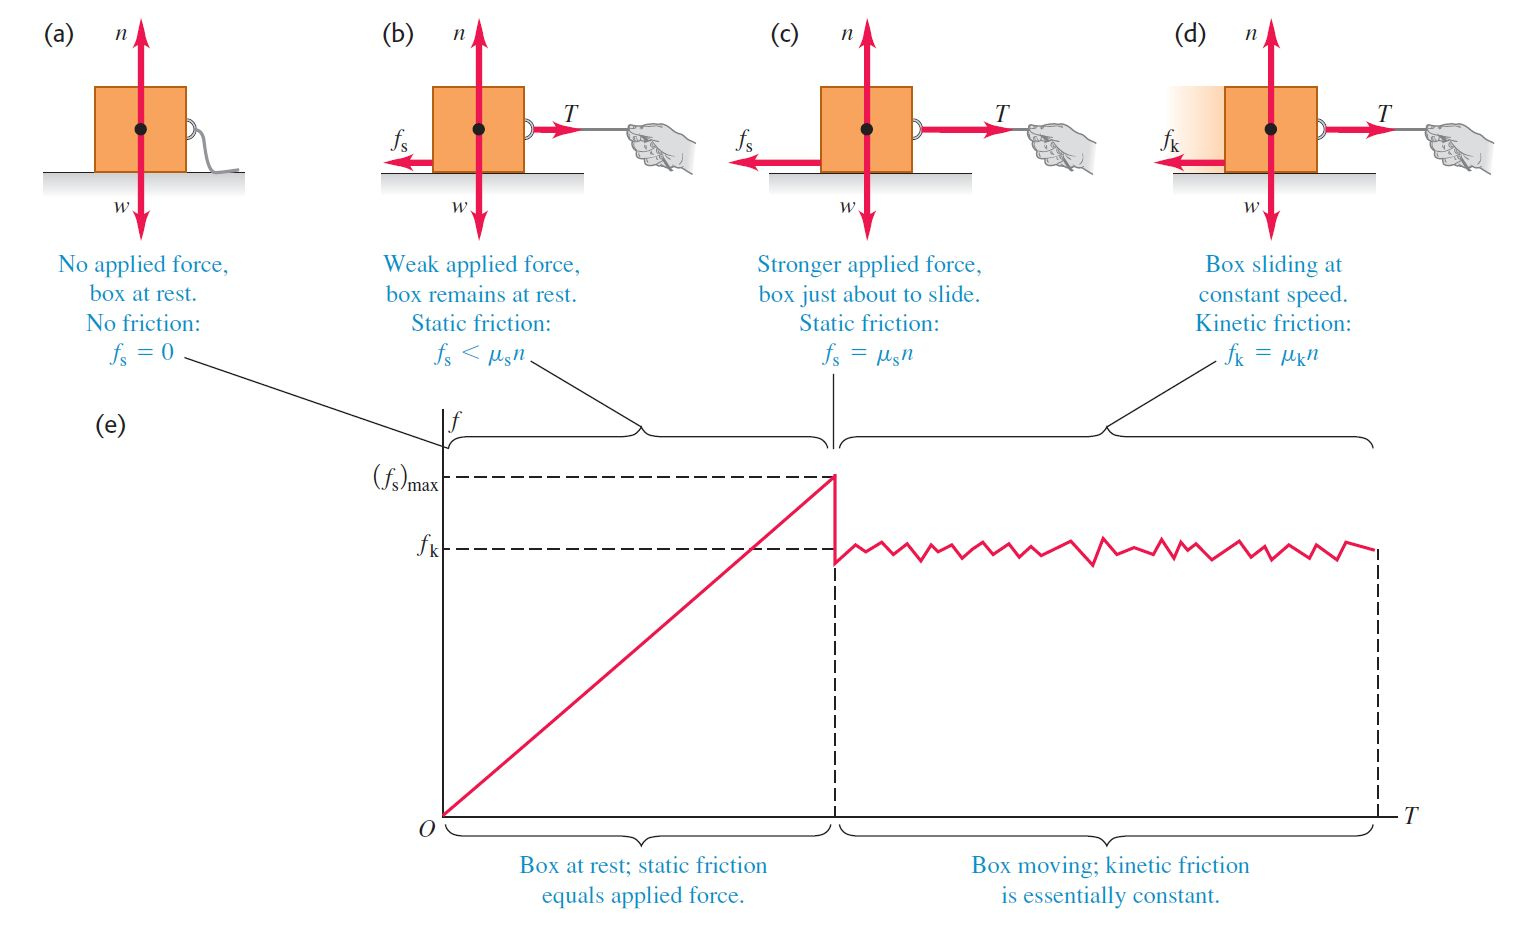
\includegraphics[width=1.\textwidth]{images/f21.jpg}
           \caption{ {\tiny Table from Sears and Zemansky's University Physics 
           with Modern Physics, 13th Edition.} }
         \end{figure}
     
               \end{frame}

    %%%%%%%%%%%%%%%%%%%%%%%%%%%%%%%%%%%%%%%%%%%%%%%%%%%%%%%%%%%%%%%%%%%






    \begin{frame}
      
      Frictional Forces
    \vspace{3mm}
    
\begin{equation}
  f_k\leq\mu_k N
\end{equation}


          \end{frame}


%%%%%%%%%%%%%%%%%%%%%%%%%%%%%%%%%%%%%%%%%%%%%%%%%%%%%%%%%%%%%%%%%%%
      




\begin{frame}
  Toboggan ride with friction 
 \vspace{3mm}

 Let’s go back to the toboggan we studied before. There is now a nonzero coefficient 
 of kinetic friction $\mu_k$ . Find the acceleration.
         
  \begin{figure}[h!]  
    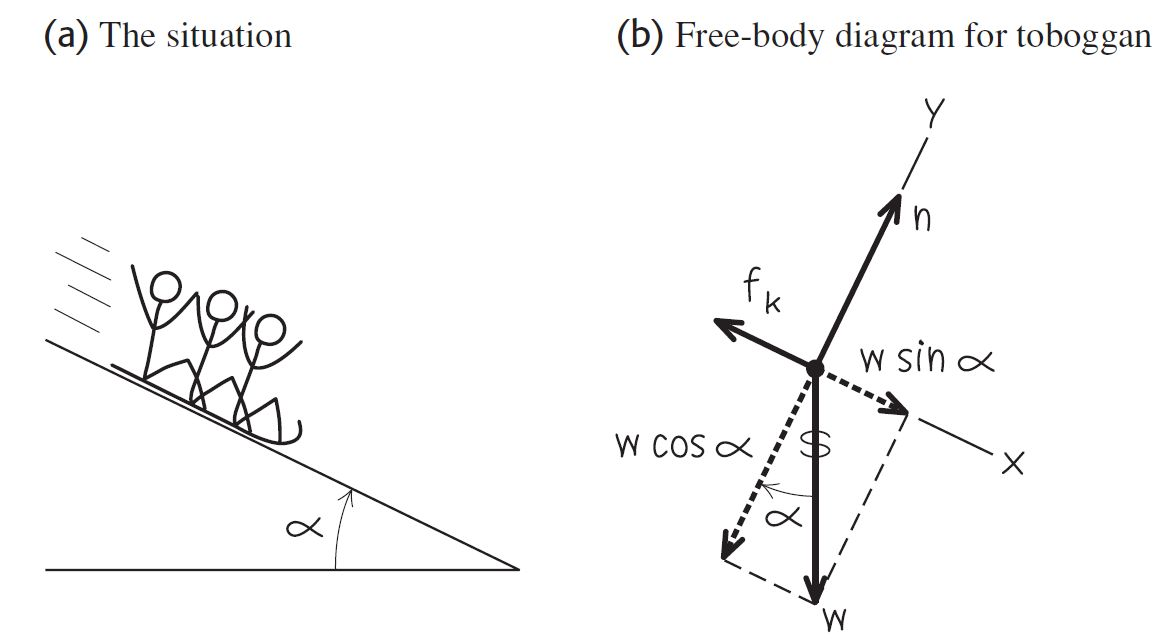
\includegraphics[width=0.7\textwidth]{images/f23.jpg}
    \caption{ {\tiny Figure from Sears and Zemansky's University Physics 
    with Modern Physics, 13th Edition.} }
  \end{figure}

        \end{frame}


%%%%%%%%%%%%%%%%%%%%%%%%%%%%%%%%%%%%%%%%%%%%%%%%%%%%%%%%%%%%%%%%%%%
      

\begin{frame}
  Toboggan ride with friction 
 \vspace{3mm}

 Let’s go back to the toboggan we studied before. There is now a nonzero coefficient 
 of kinetic friction $\mu_k$ The slope has just the right angle to make the toboggan
slide with constant velocity. Find this angle in terms of $w$ and $\mu_k$
         
  \begin{figure}[h!]  
    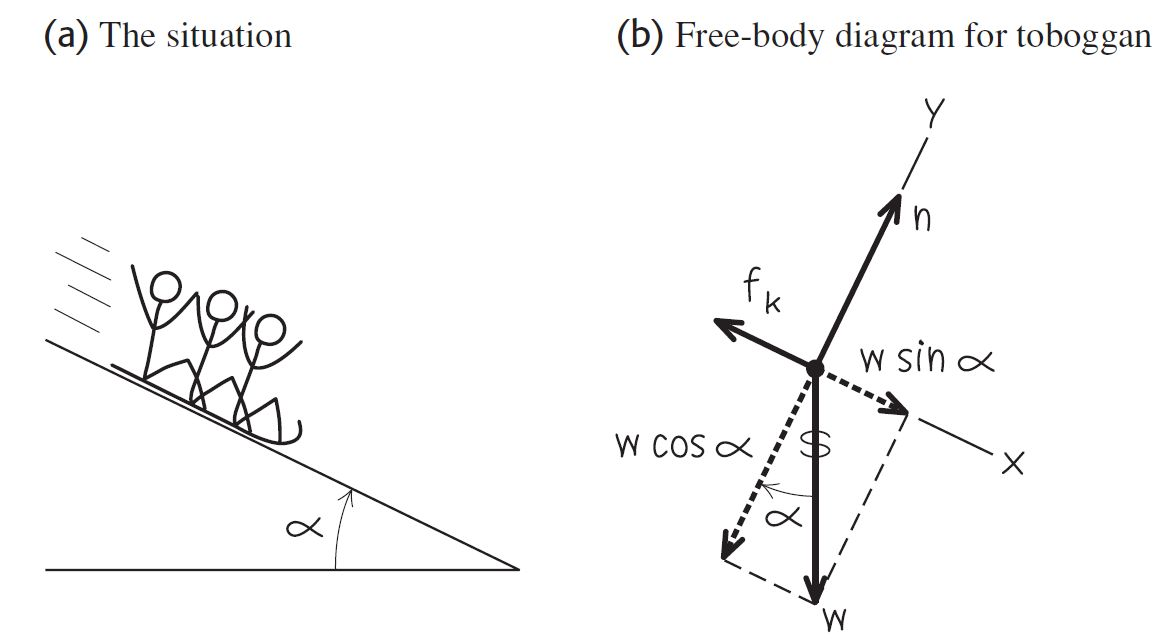
\includegraphics[width=0.7\textwidth]{images/f23.jpg}
    \caption{ {\tiny Figure from Sears and Zemansky's University Physics 
    with Modern Physics, 13th Edition.} }
  \end{figure}

        \end{frame}

%%%%%%%%%%%%%%%%%%%%%%%%%%%%%%%%%%%%%%%%%%%%%%%%%%%%%%%%%%%%%%%%%%%
      




\begin{frame}
  Fluid Resistance and Terminal Speed
 \vspace{3mm}



 \begin{columns}[c]
  \column{2in}  % slides are 3in high by 5in wide
 

  \begin{figure}[h!]  
    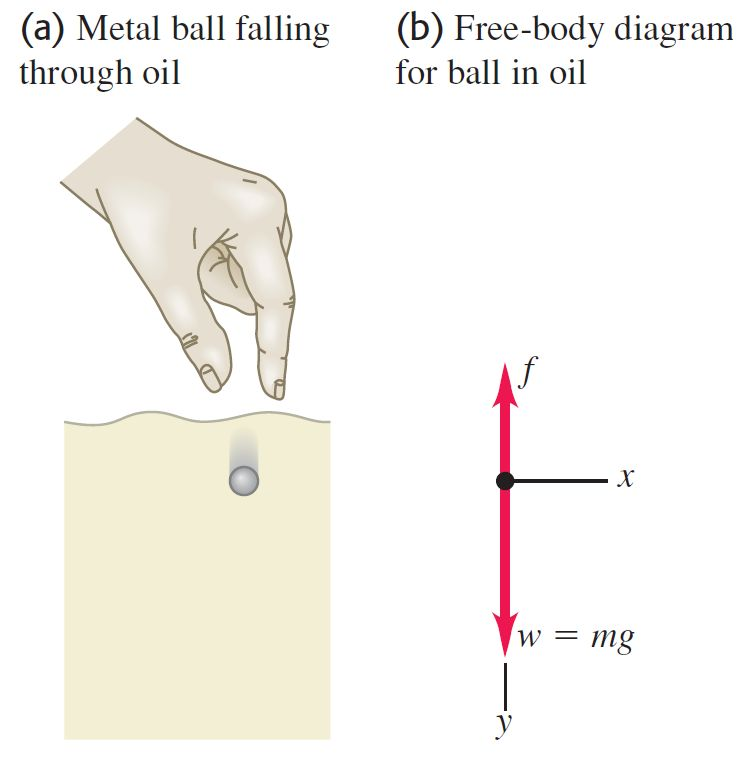
\includegraphics[width=1.\textwidth]{images/f24.jpg}
    \caption{ {\tiny Figure from Sears and Zemansky's University Physics 
    with Modern Physics, 13th Edition.} }
  \end{figure}

  \column{2in}

\begin{itemize}
  \item The \textbf{fluid resistance} is the force that a fluid exerts on a
  body moving through it.
  \pause
  \item The direction of the fluid resistance force is always opposite
  the direction of the motion.
  \pause
  \item $f=kv$ (fluid resistance at low speed).
\end{itemize}



  \end{columns}


   \end{frame}

%%%%%%%%%%%%%%%%%%%%%%%%%%%%%%%%%%%%%%%%%%%%%%%%%%%%%%%%%%%%%%%%%%%

\begin{frame}
  Fluid Resistance and Terminal Speed
 \vspace{3mm}


\begin{itemize}
  \item In this kind of motion, the force depends on the velocity, but the velocity depends also on the force.
 \pause
  \item To solve the problem we need to solve a differential equation $\rightarrow$ beyond the scope of this course.
\pause
  \item At some point the system reaches an equilibrium, there is a terminal speed. 
\end{itemize}





  
   \end{frame}





   %%%%%%%%%%%%%%%%%%%%%%%%%%%%%%%%%%%%%%%%%%%%%%%%%%%%%%%%%%%%%%%%%%%





 \begin{frame}
  Fluid Resistance and Terminal Speed
 \vspace{3mm}



 \begin{columns}[c]
  \column{2in}  % slides are 3in high by 5in wide
 

  \begin{figure}[h!]  
    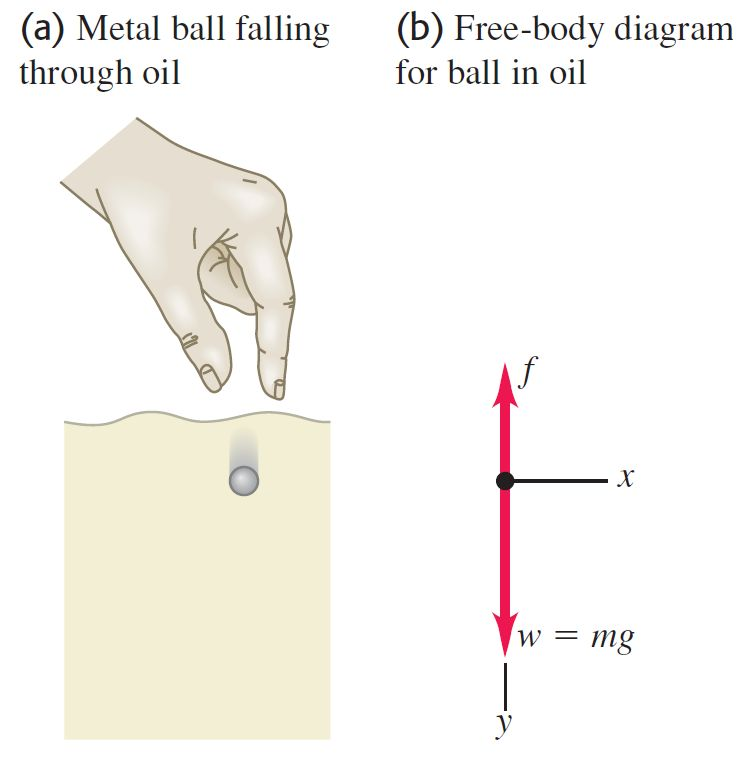
\includegraphics[width=1.\textwidth]{images/f24.jpg}
    \caption{ {\tiny Figure from Sears and Zemansky's University Physics 
    with Modern Physics, 13th Edition.} }
  \end{figure}

  \column{2in}

Second Newton's law:
\vspace{3mm}


\begin{equation}
  \sum F_y=mg-kv=ma
\end{equation}
\pause

Terminal speed?

\pause
\begin{equation*}
a=0\rightarrow v=\frac{mg}{k}
\end{equation*}

  \end{columns}


   \end{frame}


  

   %%%%%%%%%%%%%%%%%%%%%%%%%%%%%%%%%%%%%%%%%%%%%%%%%%%%%%%%%%%%%%%%%%%





 \begin{frame}
  Fluid Resistance and Terminal Speed
 \vspace{3mm}




  \begin{figure}[h!]  
    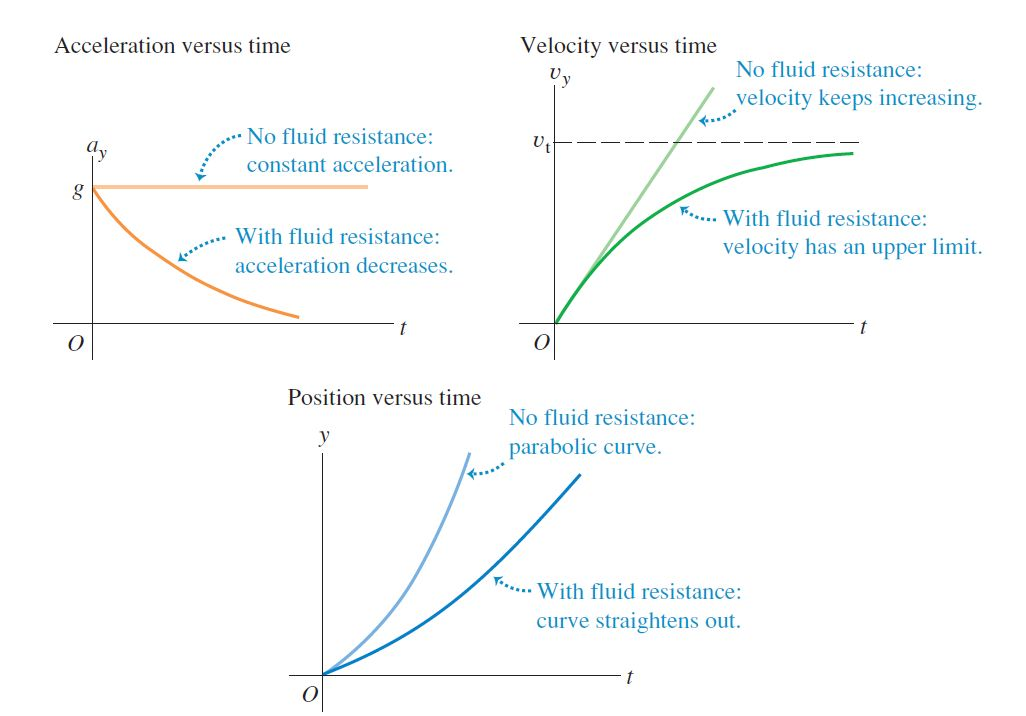
\includegraphics[width=0.8\textwidth]{images/f25.jpg}
    \caption{ {\tiny Figure from Sears and Zemansky's University Physics 
    with Modern Physics, 13th Edition.} }
  \end{figure}



   \end{frame}



   %%%%%%%%%%%%%%%%%%%%%%%%%%%%%%%%%%%%%%%%%%%%%%%%%%%%%%%%%%%%%%%%%%%





   \begin{frame}
    Rounding a banked curve
   \vspace{3mm}
  
   For a car traveling at a certain speed, it is possible to bank a curve at
   just the right angle so that no friction at all is needed to maintain the
   car’s turning radius. Then a car can safely round the curve even on
   wet ice. At what angle should the curve be banked?
  
  
    \begin{figure}[h!]  
      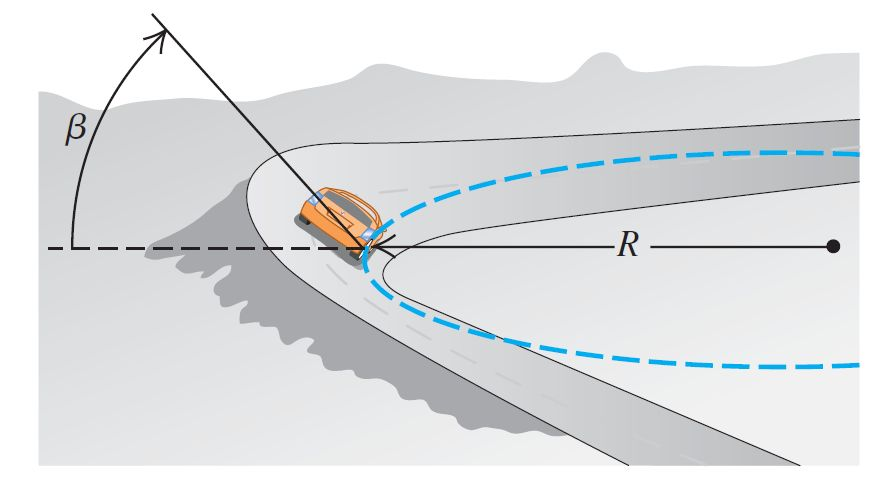
\includegraphics[width=0.5\textwidth]{images/f27.jpg}
      \caption{ {\tiny Figure from Sears and Zemansky's University Physics 
      with Modern Physics, 13th Edition.} }
    \end{figure}
  
  
  
     \end{frame}

     




        %%%%%%%%%%%%%%%%%%%%%%%%%%%%%%%%%%%%%%%%%%%%%%%%%%%%%%%%%%%%%%%%%%%





   \begin{frame}
  Motion in a vertical circle.
   \vspace{3mm}
  
   A passenger on a carnival Ferris wheel moves in a vertical circle of
   radius R with constant speed The seat remains upright during
   the motion. Find expressions for the force the seat exerts on the
   passenger at the top of the circle and at the bottom.
  
  
    \begin{figure}[h!]  
      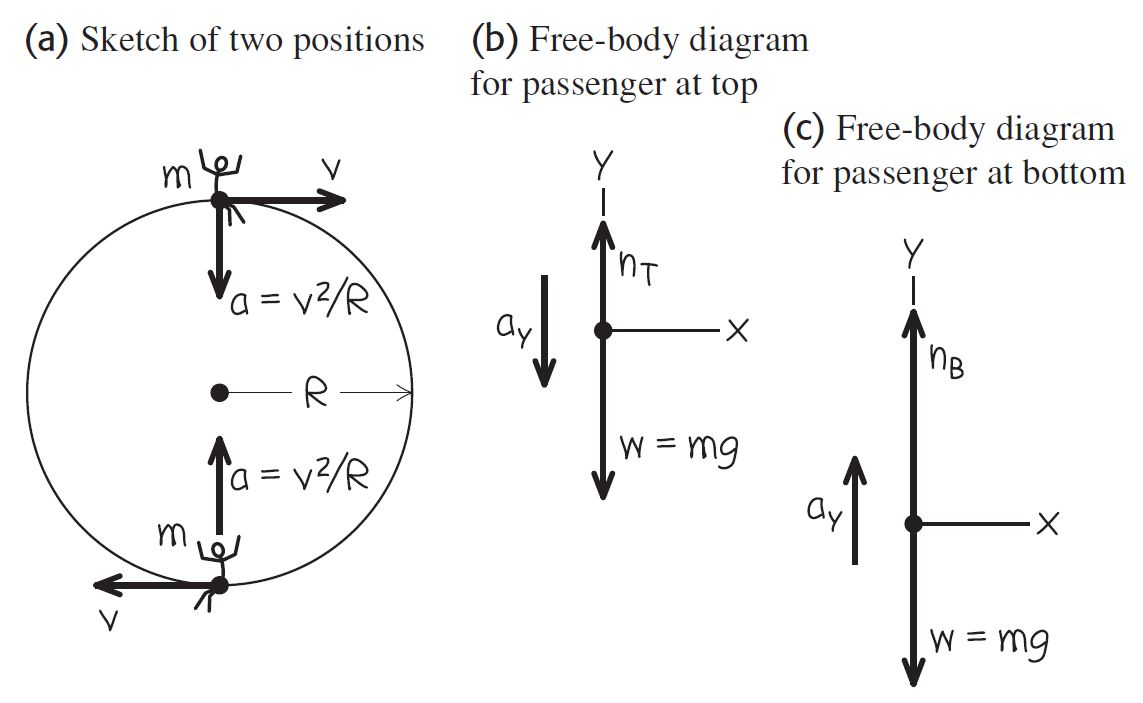
\includegraphics[width=0.8\textwidth]{images/f28.jpg}
      \caption{ {\tiny Figure from Sears and Zemansky's University Physics 
      with Modern Physics, 13th Edition.} }
    \end{figure}
  
  
  
     \end{frame}




%%%%%%%%%%%%%%%%%%%%%%%%%%%%%%%%%%%%%%%%%%%%%%%%%%%%%%%%%%%%%%%%%%%

\begin{frame}

     Test Your Understanding 
     \vspace{3mm}
     
     
     Satellites are held in orbit by the force of our planet’s gravitational attraction. 
     A satellite in a small-radius orbit moves at a higher speed than a satellite in an orbit
      of large radius. Based on this information, what you can conclude about the earth’s 
      gravitational attraction for the satellite?

      \vspace{3mm}

      \begin{itemize}
        \item It increases with increasing distance from the earth.
        \item It is the same at all distances from the earth.
        \item It decreases with increasing distance from the earth.
        \item This information by itself isn’t enough to answer the question.
      \end{itemize}

    \end{frame}





%%%%%%%%%%%%%%%%%%%%%%%%%%%%%%%%%%%%%%%%%%%%%%%%%%%%%%%%%%%%%%%%%%%











%%%%%%%%%%%%%%%%%%%%%%%%%%%%%%%%%%%%%%%%%%%%%%%%%%%%%%%%%%%%%%%%%%%
 \end{document}
%%%%%%%%%%%%%%%%%%%%%%%%%%%%%%%%%%%%%%%%%%%%%%%%%%%%%%%%%%%%%%%%%%%